\documentclass{article}
\usepackage[portuguese]{babel}
\usepackage{macros, booktabs}
\title{Tarefa 3 - MAT01050}
\author{Leonardo Suarez}
\date{\today}

\begin{document}
\maketitle

\begin{unprblm}
    Considere os dados abaixo gerados em um experimento:
    \begin{table}[h!]
    \centering
    \caption{Dados experimentais obtidos}
    \begin{tabular}{ccccccccccccc}
    \toprule
    $x$    & 0,0 & 1,0 & 1,5 & 2,3 & 2,5 & 4,0 & 5,1 & 6,0 & 6,5 & 7,0 & 8,1 & 9,0 \\
    $f(x)$ & 0,2 & 0,8 & 2,5 & 2,5 & 3,5 & 4,3 & 3,0 & 5,0 & 3,5 & 2,4 & 1,3 & 2,0 \\
    \midrule
    $x$    & 9,3 & 11,0 & 11,3 & 12,1 & 13,1 & 14,0 & 15,5 & 16,0 & 17,5 & 17,8 & 19,0 & 20,0 \\
    $f(x)$ & -0,3 & -1,3 & -3,0 & -4,0 & -4,9 & -4,0 & -5,2 & -3,0 & -3,5 & -1,6 & -1,4 & -0,1 \\
    \bottomrule
    \end{tabular}
    \end{table}

    \begin{itemize}
        \item [(1)] Escolha o polinômio de ordem inferior mais adequado para ajuste destes dados, usando o critério dos mínimos quadrados. Justifique sua escolha. Apresente o polinômio obtido. Faça um gráfico (preferencialmente contendo os pontos dados e a curva do polinômio estimado).
        \item [(2)] Assuma agora que desejasse ajustar o mesmo conjunto de dados a uma função da forma:
        \begin{equation}
            g(x) = A + B \sin\left(\frac{\pi x}{10}\right)
        \end{equation}

        Defina então a função de erro quadrático $E$ para $n = 24$:
        \begin{equation}
            E = \sum_{i=1}^{n} [g(x_i) - f(x_i)]^2 \implies E = \sum_{i=1}^{n} \left[ A + B \sin\left(\frac{\pi x_i}{10}\right) - f(x_i) \right]^2
        \end{equation} de forma a determinar os parâmetros $A$ e $B$ que minimizem $E$ (calculando as derivadas parciais de $E$ com relação a $A$ e $B$, respectivamente, e igualando a zero).

        Diante disso:
        \begin{itemize}
            \item Apresente o sistema linear obtido para determinação de $A$ e $B$;
            \item Apresente a função $g(x)$ encontrada e indique se considera o melhor ajuste o que foi obtido em (1) ou (2), justificando sua resposta.
        \end{itemize}
    \end{itemize}    
\end{unprblm}

\begin{proof}[Solução]
    \begin{itemize}
        \item [(1)] Plotando os pontos dados, observamos que eles parecem seguir um comportamento de uma função cúbica. 
        \begin{figure}[H]
            \centering
            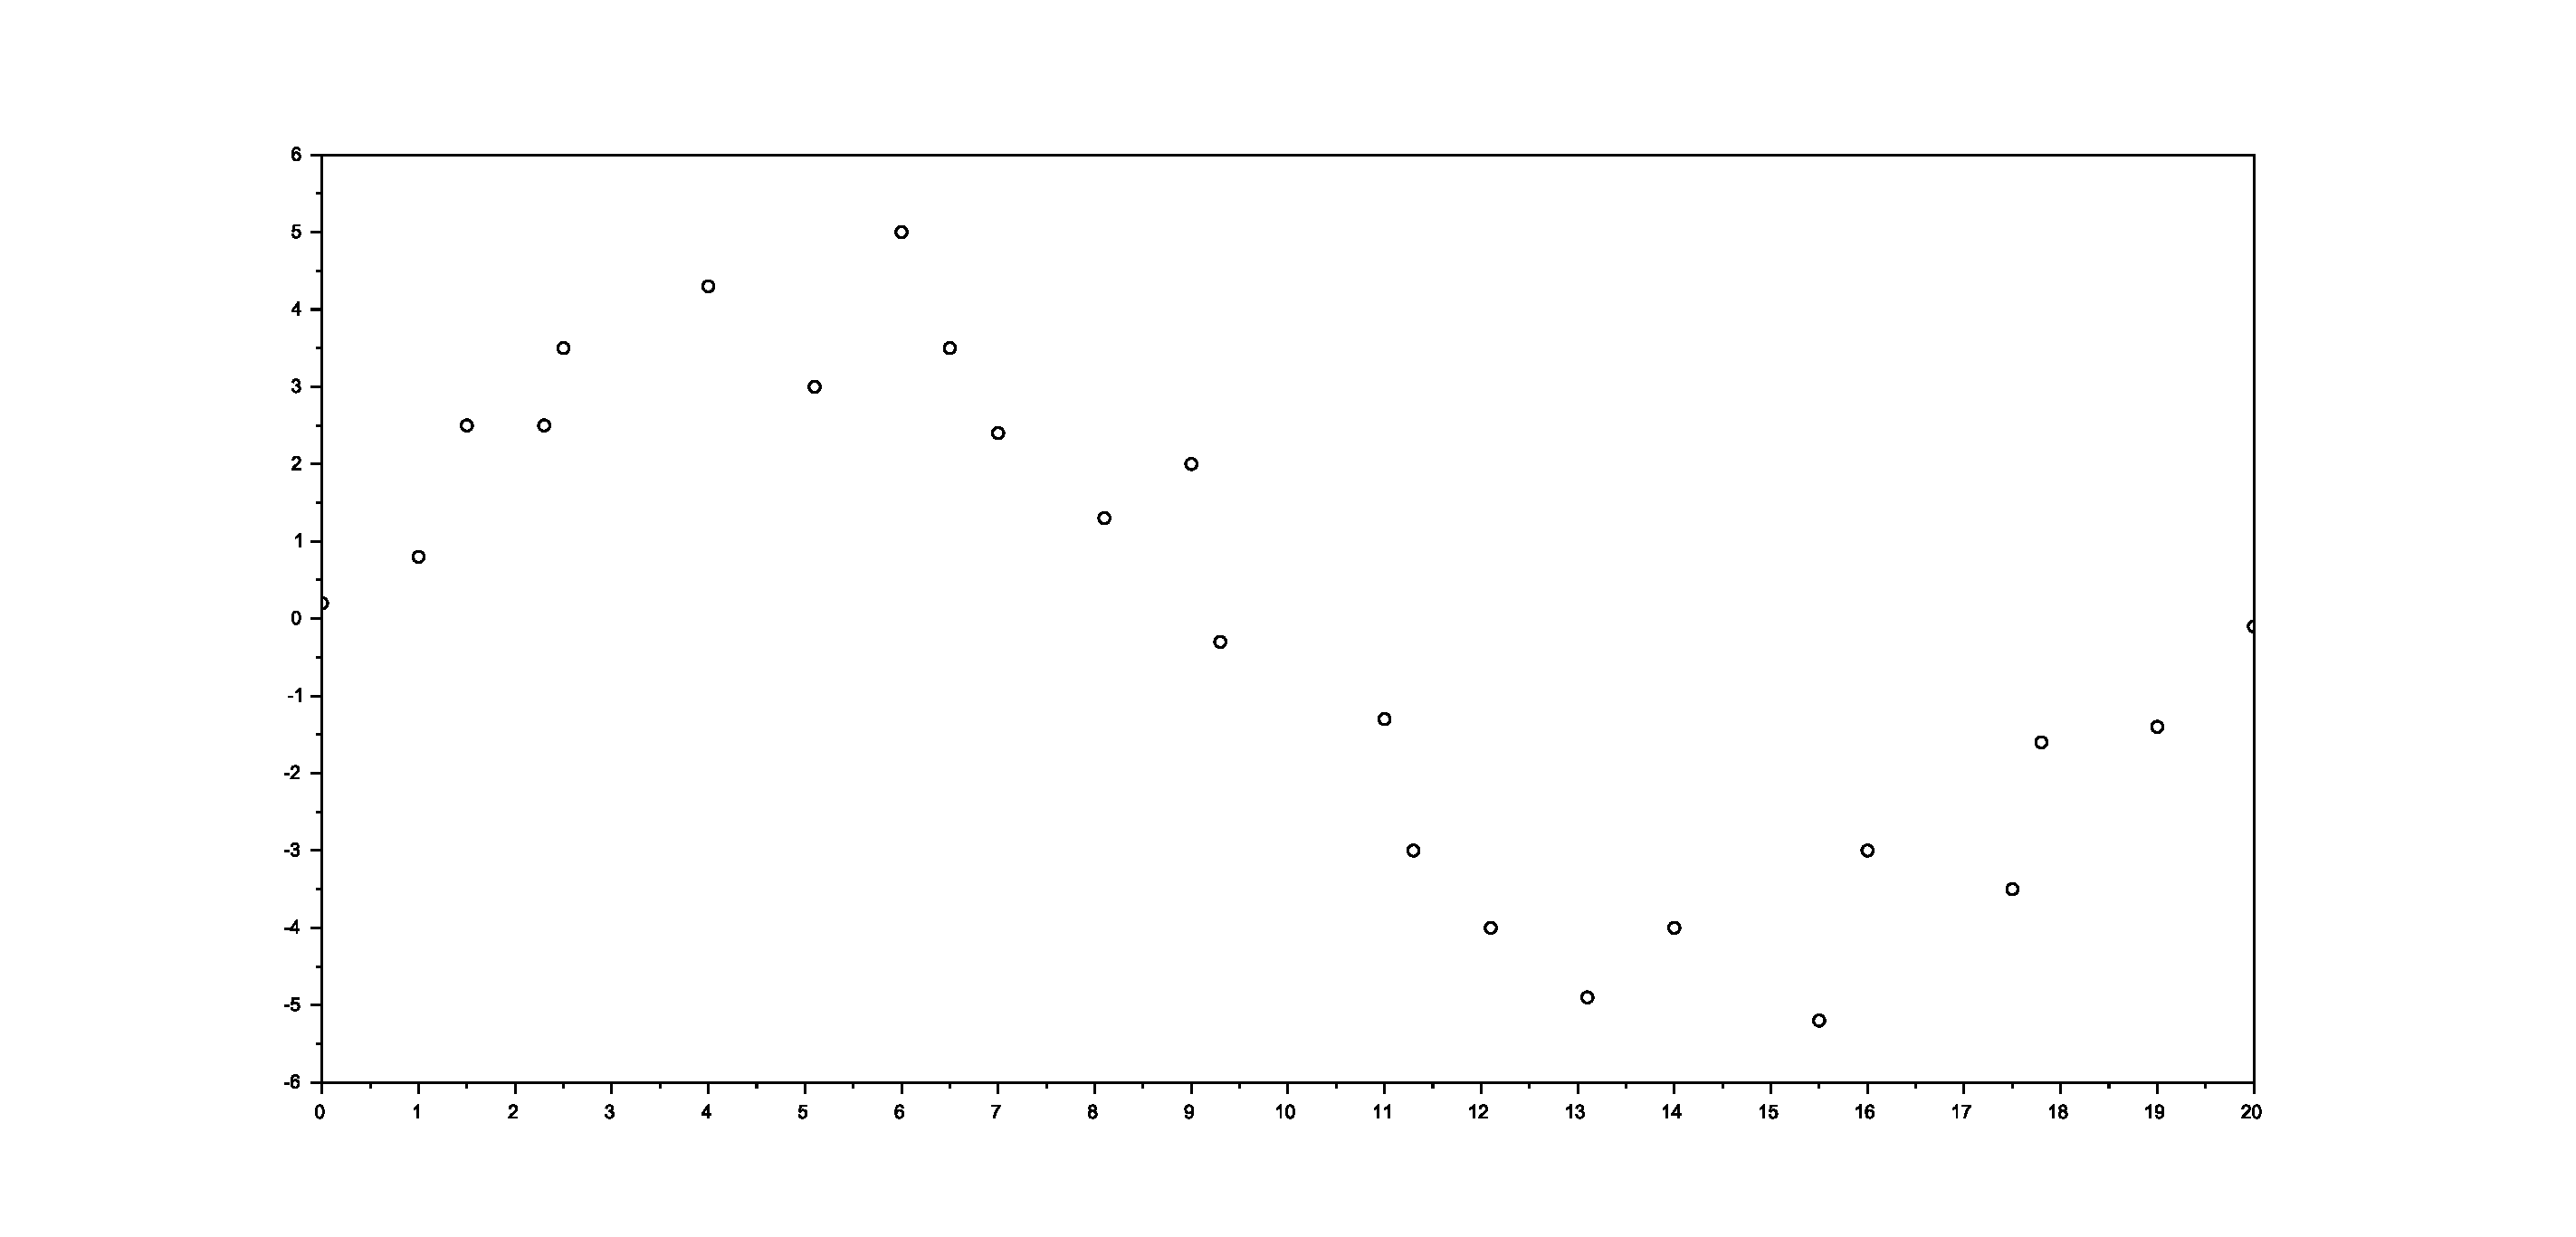
\includegraphics[width=\textwidth]{tarefa_3_dados.pdf}
            \caption{Gráfico dos pontos experimentais}
        \end{figure}

        Uma curva que se ajusta a esses pontos apresenta uma única mudança de curvatura (inflexão) perto de \(x=10\), o que é característico de um polinômio de grau 3 (que possui no máximo um ponto de inflexão). Queremos então determinar os coeficientes \(a_0, a_1, a_2, a_3\) do polinômio \(p(x) = a_0 + a_1 x + a_2 x^2 + a_3 x^3\) que minimiza o erro quadrático entre \(p(x_i)\) e \(f(x_i)\) para os dados fornecidos. O sistema linear para encontrar esses coeficientes é dado pela matriz de Vandermonde \(V_{24 \times 4}\):
        \[ Va = f(x) = \begin{bmatrix}
            1 & x_1 & x_1^2 & x_1^3 \\
            1 & x_2 & x_2^2 & x_2^3 \\
            \vdots & \vdots & \vdots & \vdots \\
            1 & x_{24} & x_{24}^2 & x_{24}^3
        \end{bmatrix} \begin{bmatrix}
            a_0 \\
            a_1 \\
            a_2 \\
            a_3
        \end{bmatrix} = \begin{bmatrix}
            f(x_1) \\
            f(x_2) \\
            \vdots \\
            f(x_{24})
        \end{bmatrix}.
        \] Resolvemos o problema de mínimos quadrados \(V a = f(x)\) usando a função \texttt{qrlstsq}, apresentada abaixo. 
        
        \begin{lstlisting}[language=Scilab, caption=Resolução do problema de mínimos quadrados usando decomposição QR]
            function [x, r] = qrlstsq(A,b)
                // solve the least-squares problem using (reduced) QR decomposition
                // input: m x n matrix A of full rank and m x 1 column vector b
                // output: solution to the least-squares problem Ax=b and the residual
                [Q,R] = qr(A); // compute the reduced QR decomposition of A
                [m,n] = size(A);
                c = Q'*b;
                
                // solve the upper-triangular system Rx=c by back substitution
                x = zeros(n,1);
                x(n) = c(n) / R(n,n);
                for j = n-1:-1:1
                    x(j) = (c(j) - R(j,j+1:n)*x(j+1:n)) / R(j,j);
                end
                
                // compute the residual r = b-Ax
                r = b - A*x;
            endfunction
        \end{lstlisting}

        O polinômio obtido é 
        \[
            p(x) = -0.3593472 +2.3051112x -0.3531901x^2 +0.0120602x^3.
        \] Plotamos a curva de \(p(x)\) (em azul) no gráfico \ref{fig:ajuste}, juntamente com os pontos experimentais.
        \item [(2)] Computamos as derivadas parciais de \(E\) em relação a \(A\) e \(B\) e igualamos a zero:
        \begin{align*}
            \frac{\partial E}{\partial A} &= 2 \sum_{i=1}^{n} \left[ A + B \sin\left(\frac{\pi x_i}{10}\right) - f(x_i) \right] = 0, \\
            \frac{\partial E}{\partial B} &= 2 \sum_{i=1}^{n} \left[ A + B \sin\left(\frac{\pi x_i}{10}\right) - f(x_i) \right] \sin\left(\frac{\pi x_i}{10}\right) = 0.
        \end{align*} Reorganizando os termos, obtemos o sistema linear:
        \begin{align*}
            \begin{bmatrix}
                n & \displaystyle\sum_{i=1}^{n} \sin\left(\frac{\pi x_i}{10}\right) \\
                \displaystyle\sum_{i=1}^{n} \sin\left(\frac{\pi x_i}{10}\right) & \displaystyle\sum_{i=1}^{n} \sin^2\left(\frac{\pi x_i}{10}\right)
            \end{bmatrix} \begin{bmatrix}
                A \\
                B
            \end{bmatrix} = \begin{bmatrix}
                \displaystyle\sum_{i=1}^{n} f(x_i) \\
                \displaystyle\sum_{i=1}^{n} f(x_i) \sin\left(\frac{\pi x_i}{10}\right)
            \end{bmatrix}.
        \end{align*}

        Resolvemos esse sistema com o comando \texttt{\textbackslash} (backslash) do \texttt{Scilab} e encontramos \(A = -0.2583126\) e \(B = 4.3250839\). Assim, a função \(g(x)\) é dada por
        \begin{equation}
            g(x) = -0.2583126 + 4.3250839 \sin\left(\frac{\pi x}{10}\right).
        \end{equation}

        Plotamos a função \(g(x)\) (em vermelho) no gráfico \ref{fig:ajuste}, juntamente com os pontos experimentais e o polinômio \(p(x)\) (em azul).
        
        \begin{figure}[H]
            \centering
            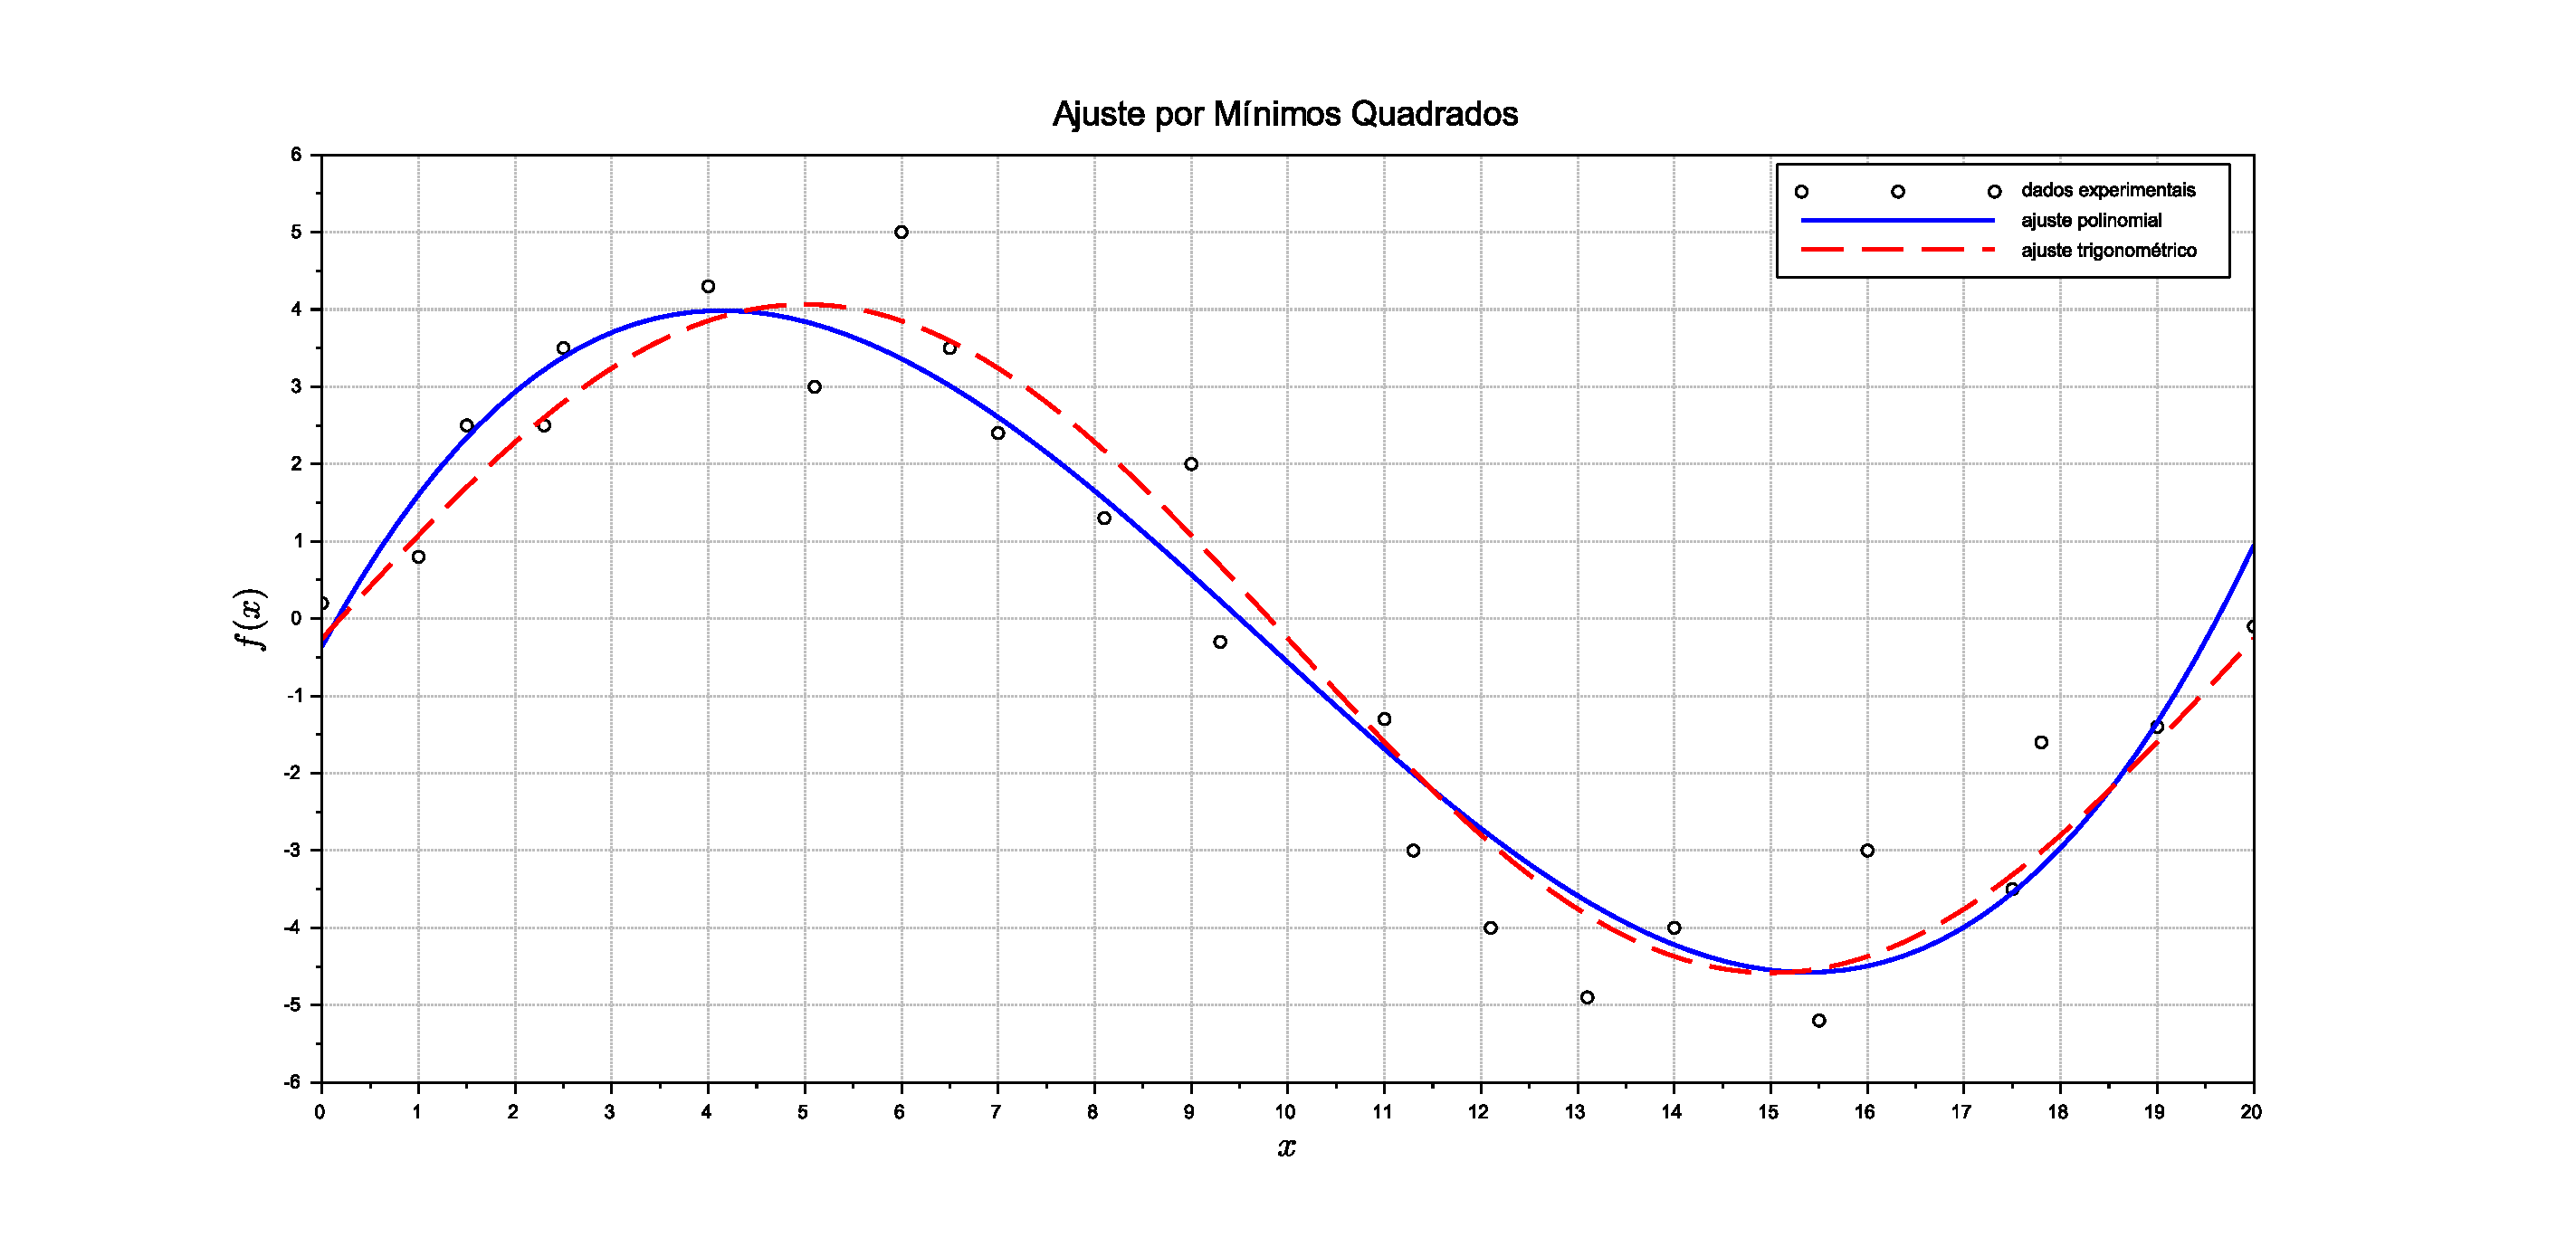
\includegraphics[width=\textwidth]{tarefa_3_ajuste.pdf}
            \caption{Gráfico dos ajustes polinomial e trigonométrico}
            \label{fig:ajuste}
        \end{figure}

        Observamos que ambos os ajustes capturam a tendência geral dos dados. Para compará-los, podemos calcular o erro quadrático \(E\) para cada ajuste. O erro quadrático para o polinômio \(p(x)\) é dado por
        \begin{equation}
            E_p = \sum_{i=1}^{n} [p(x_i) - f(x_i)]^2,
        \end{equation} e para a função \(g(x)\) é dado por
        \begin{equation}
            E_g = \sum_{i=1}^{n} [g(x_i) - f(x_i)]^2.
        \end{equation} Calculando esses erros, encontramos \(E_p = 18.101050\) e \(E_g = 15.386139\). Além disso, o ajuste trigonométrico precisou de apenas 2 parâmetros, enquanto o ajuste polinomial precisou de 4 parâmetros. Considerando esses dois fatores, podemos concluir que o ajuste trigonométrico é melhor do que o ajuste polinomial para os dados fornecidos.
    \end{itemize}
\end{proof}

\end{document}